% !TEX encoding = UTF-8
% !TEX TS-program = pdflatex
% !TEX root = ../thesis.tex

%************************************************
\chapter{Results and Discussion}\label{chap:six}
%************************************************

In this chapter, we present the main results of this PhD thesis. First, we show results for the total and differential top-bottom interference contributions to the gluon-gluon-fusion Higgs-production cross section in both the 4\acs{FS} and the 5\acs{FS}. We then compare the results in the \acs{OS} and the \MS\ renormalization schemes for the top- and bottom-quark masses. We also provide pure-top-quark-mass effects and, finally, compare our findings with other works.

We use two scale choices; for fully-inclusive cross section we use the central scale of $\mu = m_H/2$, as it shows very good perturbative convergence as explained in Section~\ref{subsec:4:scale_uncertainties}. In differential cross sections we use the dynamic scale
\begin{equation}
\mu = \frac{H_T}{2} \equiv \frac{1}{2} \left( \sqrt{m_H^2 + p_T^2} + \sum_i p_{i, T} \right),
\label{eq:6:mu_dynamic}
\end{equation}
where $p_T$ is the transverse momentum of the Higgs, and $p_{i, T}$ is the transverse momentum of the $i$-th final state parton. The scale was chosen on the one hand to match previous studies~\cite{Lindert:2017pky, Bonciani:2022jmb, Jones:2018hbb}, but also to improve perturbative convergence at large $p_T$, where the Higgs mass alone is no longer the natural scale. This is evident for example in the phase-space measure of Eq.~\eqref{eq:4:PS_measure}, which shows that at large transverse momentum we encounter logarithms of the form $\log (\mu^2/s)$. So because $H_T$ is the minimum partonic center of mass energy (see Eq.~\eqref{eq:4:smin}), it will result in better convergence at large $p_T$.

Unless specified otherwise, we follow the computational setup described in the \hyperref[chap:notation_and_conventions]{conventions}.
\section{Total Cross Section}
\subsection{Effects of Finite Top-Quark Masses}
As mentioned before, the finite top quark mass effects on the Higgs production cross section in the \acs{OS}-scheme have already been studied in Ref.~\cite{Czakon:2021yub}. Here we reproduce the result computed therein and complement them with scale uncertainties. We further provide results for additional center of mass energies. The results are displayed in Tab.~\ref{tab:6:t-HEFT}. Moreover, we compare the \acs{rHTL} and the full \acs{QCD} cross sections in the various partonic channels in Fig.~\ref{fig:4:HTL_accuracy} and Tab.~\ref{tab:4:finite_top_quark_mass_effects}.
\begin{table}[t]
\centering
\begin{tabular}{cccc}
Order  &  $\sigma_\text{rHTL}$ [pb] & $(\sigma_t - \sigma_\text{rHTL})$ [pb]  &  $(\sigma_t - \sigma_\text{rHTL})/\sigma_\text{rHTL}$ [\%]  \\
\hline
\hline
\multicolumn{4}{c}{$\sqrt{s}=7$~TeV}\\
\hline
$\mathcal{O}(\alpha_s^2)$ & $+5.85$ & -- &  \\
LO & $5.85^{+1.56}_{-1.11}$ & -- & --  \\
\hline
$\mathcal{O}(\alpha_s^3)$ & $+7.14$ & $-0.0604$ &  \\
NLO & $12.99^{+2.89}_{-2.14}$ & $-0.0604^{+0.021}_{-0.037}$ & $-0.5$  \\
\hline
$\mathcal{O}(\alpha_s^4)$ & $+3.28$ & $+0.0386(2)$ &  \\
NNLO & $16.27^{+1.45}_{-1.61}$ & $-0.0218(2)^{+0.035}_{-0.009}$ & $-0.1$  \\
\hline
\hline
\multicolumn{4}{c}{$\sqrt{s}=8$~TeV}\\
\hline
$\mathcal{O}(\alpha_s^2)$ & $+7.39$ & -- &  \\
LO & $7.39^{+1.98}_{-1.40}$ & -- & --  \\
\hline
$\mathcal{O}(\alpha_s^3)$ & $+9.14$ & $-0.0873$ &  \\
NLO & $16.53^{+3.63}_{-2.73}$ & $-0.0873^{+0.030}_{-0.052}$ & $-0.5$  \\
\hline
$\mathcal{O}(\alpha_s^4)$ & $+4.19$ & $+0.0523(2)$ &   \\
NNLO & $20.72^{+1.84}_{-2.06}$ & $-0.0350(2)^{+0.048}_{-0.013}$ & $-0.2$  \\
\hline
\hline
\multicolumn{4}{c}{$\sqrt{s}=13$~TeV}\\
\hline
$\mathcal{O}(\alpha_s^2)$ & $+16.30$ & -- &   \\
LO & $16.30^{+4.36}_{-3.10}$ & -- & --  \\
\hline
$\mathcal{O}(\alpha_s^3)$ & $+21.14$ & $-0.303$ &  \\
NLO & $37.44^{+8.42}_{-6.29}$ & $-0.303^{+0.10}_{-0.17}$ & $-0.8$  \\
\hline
$\mathcal{O}(\alpha_s^4)$ & $+9.72$ & $+0.147(1)$ &   \\
NNLO & $47.16^{+4.21}_{-4.77}$ & $-0.156(1)^{+0.13}_{-0.03}$ & $-0.3$  \\
\hline
\hline
\multicolumn{4}{c}{$\sqrt{s}=13.6$~TeV}\\
\hline
$\mathcal{O}(\alpha_s^2)$ & $+17.47$ & -- &   \\
LO & $17.47^{+4.67}_{-3.32}$ & -- & --  \\
\hline
$\mathcal{O}(\alpha_s^3)$ & $+22.76$ & $-0.338$ &   \\
NLO & $40.23^{+9.07}_{-6.77}$ & $-0.338^{+0.11}_{-0.18}$ & $-0.8$  \\
\hline
$\mathcal{O}(\alpha_s^4)$ & $+10.47$ & $+0.162(1)$ &  \\
NNLO & $50.70^{+4.53}_{-5.14}$ & $-0.176(1)^{+0.14}_{-0.03}$ & $-0.3$  \\
\hline
\hline
\multicolumn{4}{c}{$\sqrt{s}=14$~TeV}\\
\hline
$\mathcal{O}(\alpha_s^2)$ & $+18.26$ & -- &   \\
LO & $18.26^{+4.88}_{-3.47}$ & -- & --  \\
\hline
$\mathcal{O}(\alpha_s^3)$ & $+23.86$ & $-0.362$ &   \\
NLO & $42.12^{+9.51}_{-7.10}$ & $-0.362^{+0.12}_{-0.20}$ & $-0.9$  \\
\hline
$\mathcal{O}(\alpha_s^4)$ & $+10.98$ & $+0.171(1)$ &   \\
NNLO & $53.10^{+4.75}_{-5.39}$ & $-0.191(1)^{+0.15}_{-0.04}$ & $-0.4$  \\
\hline
\end{tabular}
\caption{Total gluon-gluon fusion cross section in the \acs{rHTL} and the pure-top-quark-mass effects for a selection of hadronic center of mass energies relevant for \acs{LHC} phenomenology. The top-quark mass is renormalized in the \acs{OS}-scheme. The computational setup is described in the \hyperref[chap:notation_and_conventions]{conventions}. The scale uncertainties are determined with seven-point variation.}
\label{tab:6:t-HEFT}
\end{table}
As discussed earlier, the \acs{rHTL} provides an excellent approximation of the cross section. By looking at Fig.~\ref{fig:4:HTL_accuracy}, we see that this is especially true for the gluon-gluon channel, whereas the other channels show discrepancies of $\BigO{10}\%$. The dominance of the gluon-gluon channel then results in the remarkable accuracy of the \acs{rHTL} when combining all partonic channels, yielding approximations with sub-percent precision. We observe that the \acs{NNLO} correction of $\sigma_t - \sigma_{\text{rHTL}}$ has the opposite sign and roughly half the magnitude of the \acs{NLO} correction. The lower scale uncertainties are reduced drastically by a factor of 4--6 going from \acs{NLO} to \acs{NNLO}, while the upper uncertainties increase slightly.

In Tab.~\ref{tab:6:topSchemeDifference} we show the difference between top-quark induced gluon-gluon fusion cross section computed with a top-quark mass defined in the \MS- and the \acs{OS}-scheme. Based on the previously known \acs{LO} and \acs{NLO} order results, it was conjectured that the renormalization scheme of the top-quark mass has little effect on the cross section. We find this trend continued at \acs{NNLO}, where the difference amounts to just $-0.01$~pb or $0.2$\textperthousand\ at 13~TeV. Based on our findings, we conclude that the scale uncertainties severely overestimate the uncertainty of the difference. The scale uncertainties themselves decrease slightly going from \acs{NLO} to \acs{NNLO}.
\begin{table}[t]
  \centering
  \begin{tabular}{cc}
  \hline
      Order & $(\sigma_t^{\overline{\mathrm{MS}}} - \sigma_t^{\mathrm{OS}})$ [pb] \\
  \hline
  \hline
  \multicolumn{2}{c}{$\sqrt{s}=13$~TeV} \\
  \hline
  $\mathcal{O}(\alpha_s^2)$     & $-0.04$ \\
  LO & $-0.04^{+0.12}_{-0.17}$ \\
  \hline
  $\mathcal{O}(\alpha_s^3)$ & $+0.02$ \\
  NLO & $-0.02^{+0.14}_{-0.30}$ \\
  \hline
  $\mathcal{O}(\alpha_s^4)$ & $+0.01$ \\
  NNLO & $-0.01^{+0.12}_{-0.24}$ \\
  \hline
  \end{tabular}
\caption{Difference of cross sections for Higgs production through a closed top-quark loop with the top-quark mass defined either in the $\overline{\mathrm{MS}}$ or the OS scheme. The results are computed for LHC @ 13 TeV using the computational setup is described in the \hyperref[chap:notation_and_conventions]{conventions}. The scale uncertainties are determined with seven-point variation.}
\label{tab:6:topSchemeDifference}
\end{table}

Lastly, we compare the pure-top-quark effects between the 4 and 5\acs{FS}. In both schemes, the Higgs boson couples exclusively to the top quark; but the two schemes differ in the treatment of the bottom-quark mass. The results are displayed in Tab.~\ref{tab:6:t-rHTL_4vs5FS}.
\begin{table}[t]
\centering
\begin{tabular}{ccc}
  \hline
  Order & \multicolumn{2}{c}{$(\sigma_{t} - \sigma_\text{rHTL})$ [pb]} \\
  \hline
  \hline
  \multicolumn{3}{c}{$\sqrt{s}=13$~TeV} \\
  \hline
  & 5FS & 4FS \\
  & $m_t = 173.06$ GeV &  $m_t = 173.06$ GeV \\
  & & $\overline{m}_b(\overline{m}_b)=4.18$ GeV\\
  \hline
  LO & - & - \\
  \hline
  $\mathcal{O}(\alpha_s^3)$ & $-0.30$  &  $-0.27$ \\
  NLO & $-0.30^{+0.10}_{-0.17}$ & $-0.27^{+0.09}_{-0.16}$ \\
  \hline
  $\mathcal{O}(\alpha_s^4)$ & $+0.14$ & $+0.12$ \\
  NNLO & $-0.16^{+0.13}_{-0.03}$ & $-0.15^{+0.10}_{-0.02}$\\
  \hline
  \end{tabular}
\caption{Effect of the finite top-quark mass on the gluon-gluon fusion cross section in the 4 and 5\acs{FS}. The top-quark mass is defined in the \acs{OS}-scheme, while the bottom-quark mass is defined in the \MS-scheme. The results are computed for LHC @ 13 TeV using the computational setup described in the \hyperref[chap:notation_and_conventions]{conventions}. The scale uncertainties are determined with seven-point variation.}
\label{tab:6:t-rHTL_4vs5FS}
\end{table}
The differences between the two schemes are insignificant, reaching $0.03$~pb at \acs{NLO} and $0.01$~pb at \acs{NNLO} at a center of mass energy of 13~TeV. At \acs{NLO} the only difference between the computations is the used \acs{PDF} set and the additional $qg \longrightarrow Hq$ channel in the 5\acs{FS}. Only at \acs{NNLO} do we have explicit dependence on the bottom-quark mass in the 4\acs{FS}, which does however not give rise to significant deviations; in fact the \acs{NNLO} results show even smaller deviations between the two schemes. We stress however that the \acs{rHTL} cross sections themselves decrease by a significant $-1.16\ \mathrm{pb}$ when moving from the 5 to the 4\acs{FS} (see Tab.~\ref{tab:6:rHTL_4fs}).

\subsection{Effects of Finite Bottom-Quark Masses}
Tab.~\ref{tab:6:top-bottom} shows one of the major findings of this work: the top-bottom interference contribution to the gluon-gluon fusion cross section at \acs{NNLO}. Herein, we compare various computational setups, including results computed with \MS- and \acs{OS}-renormalized bottom- and top-quark masses, as well as results in the 5 and 4\acs{FS}.
\begin{landscape}
\begin{table*}[t]
\centering
\begin{tabular}{cccccc}
\hline
Order & \multicolumn{5}{c}{$\sigma_{t\times b}$ [pb]} \\
\hline
\hline
\multicolumn{6}{c}{$\sqrt{s}=13$~TeV} \\
\hline
& 5FS & 5FS  & 5FS & 4FS & 5FS \\
& $m_t = 173.06$ GeV & $m_t = 173.06$ GeV &  $\overline{m}_t(\overline{m}_t) = 162.7$ GeV &  $m_t = 173.06$ GeV & $m_t = 173.06$ GeV \\
& $\overline{m}_b(\overline{m}_b) = 4.18$ GeV & $m_b = 4.78$ GeV & $\overline{m}_b(\overline{m}_b) = 4.18$ GeV & $\overline{m}_b(\overline{m}_b)=4.18$ GeV & $m_b = 4.78$ GeV\\
& & & & & $Y_b = \overline{m}_b/v$ \\
\hline
$\mathcal{O}(\alpha_s^2)$ & $-1.11$ & $-1.98$ & $-1.12$ & $-1.15$ & $-1.223$ \\
LO & $-1.11^{+0.28}_{-0.43}$ & $-1.98^{+0.38}_{-0.53}$  & $-1.12^{+0.28}_{-0.42}$ & $-1.15^{+0.29}_{-0.45}$ & $-1.223^{+0.29}_{-0.44}$ \\
\hline
$\mathcal{O}(\alpha_s^3)$ & $-0.65$ & $-0.44$ & $-0.64$ & $-0.66$ & $-0.623(1)$ \\
NLO & $-1.76^{+0.27}_{-0.28}$ & $-2.42^{+0.19}_{-0.12}$ & $-1.76^{+0.27}_{-0.28}$ & $-1.81^{+0.28}_{-0.30}$ & $-1.85^{+0.26}_{-0.26}$ \\
\hline
$\mathcal{O}(\alpha_s^4)$ & $+0.02$ & $+0.43$ & $-0.02$ & $-0.02$ & $+0.019(5)$ \\
NNLO & $-1.74(2)^{+0.13}_{-0.03}$ & $-1.99(2)^{+0.29}_{-0.15}$ & $-1.78(1)^{+0.15}_{-0.03}$ & $-1.83(2)^{+0.14}_{-0.03}$ & $-1.83(1)^{+0.08}_{-0.03}$\\
\hline
\end{tabular}
\caption{Top-bottom interference contribution to the gluon-gluon fusion cross section for various computational setups. The results are computed for LHC @ 13 TeV using the computational setup is described in the \hyperref[chap:notation_and_conventions]{conventions}. The scale uncertainties are determined with seven-point variation. Numbers in parentheses indicate the \acs{MC} uncertainties on the last provided digit.}
\label{tab:6:top-bottom}
\end{table*}
\end{landscape}

Using an \MS\ renormalized bottom-quark mass, an \acs{OS} renormalized top-quark mass, and the 5\acs{FS}, we find that the central value is not shifted significantly going from \acs{NLO} to \acs{NNLO}. The result is therefore consistent within the previously estimated scale uncertainty bands. The latter are reduced significantly in this setup. The upwards scale variation is halved, reaching a precision of $7\%$ whereas the lower uncertainty is reduced even further to about $2\%$. Overall, we observe a good perturbative convergence with this setup.

When the top-quark mass is renormalized in the \MS-scheme instead (3rd column of Tab.~\ref{tab:6:top-bottom}), we find only minor changes in the results. This is true both for the central value and the associated scale uncertainties. This aligns with our earlier observation for the pure-top-quark-mass effects, which also displayed very little dependence on the top-quark mass renormalization scheme.

The situation is very different for the renormalization scheme of the bottom-quark mass. At \acs{LO}, the cross sections in the two renormalization schemes differ by almost $80\%$. At this order, the only difference during the computation is the numerical value of the bottom-quark mass. The \acs{OS}-mass of the bottom quark is $m_b = 4.78\ \text{GeV}$, whereas the \MS-mass at the central scale can be read off Fig.~\ref{fig:5:running} and reads about $\overline{m}_b(m_H/2) = 3.0\ \text{GeV}$. The large difference at \acs{LO} is therefore explained by the large discrepancy of the two mass values and the fact that the Higgs-gluon form factor shows a strong quadratic dependence on the quark mass in the \acs{HEL} (see Eq.~\eqref{eq:4:C0_HEL}). In principle, the difference should be mitigated when including higher orders in perturbation theory. However, the poor perturbative convergence of the \MS-\acs{OS}-mass relation in Eq.~\eqref{eq:5:mbOS_mbMS_5FS} often averts such mitigations in practice. Indeed, although we observe that the gap between the \MS- and \acs{OS}-results is reduced significantly, the results in the \acs{OS}-scheme are unreliable, as the \acs{NNLO} correction has nearly the same magnitude as the \acs{NLO} correction but comes with the opposite sign. Alternating corrections of similar magnitude are a typical indicator of bad perturbative convergence. The \acs{NNLO} corrections also lie outside the previously estimated uncertainty band. Additionally, we find that the scale uncertainties actually increase going from \acs{NLO} to \acs{NNLO}, giving us further evidence that the cross section does not stabilize in the \acs{OS}-scheme. The main conclusion here is that the cross section results with an \acs{OS}-renormalized bottom-quark mass are not trustworthy. The \acs{NNLO} predictions therefore allowed us to eliminate the scheme-uncertainty previously associated with the gluon-gluon fusion cross section, by conclusively demonstrating that the \MS-scheme performs better in this instance.

To further investigate the origin of the improvements of the perturbative convergence in the \MS-scheme, we also computed results in a mixed renormalization scheme, where the bottom-quark mass is renormalized in the \acs{OS}-scheme, but the Yukawa coupling of the Higgs and the bottom-quark is renormalized in the \MS-scheme. We stress that this scheme is formally inconsistent, since in the \acs{SM}, the Yukawa couplings are set by the mass via
\begin{equation}
Y = \frac{m}{v}.
\end{equation}
Hence, the renormalization constant of the Yukawa coupling is fixed by those of the mass and the \acs{VEV}. With the inclusion of electroweak corrections, this can result in problems of gauge invariance, but since our considerations are limited to \acs{QCD} corrections, we can ignore these for our purposes. The results are much simpler to derive from the \acs{OS} results than when using the \MS-scheme consistently, because the Yukawa coupling only enters our cross section linearly, meaning that the derivatives in Eq.~\eqref{eq:5:MMS_to_MOS} are trivial, and the perturbative corrections can be obtained via
\begin{equation}
\begin{split}
\sigma^{(0)}_{t\times b, \text{Mixed}} &= \frac{\overline{m}_b}{m_b} \sigma^{(0)}_{t\times b, \text{OS}} \\
\sigma^{(1)}_{t \times b, \text{Mixed}} &= \frac{\overline{m}_b}{m_b} \left[ \sigma^{(1)}_{t \times b, \text{OS}} + c_1^{(5,5)} \frac{\alphas}{\pi} \sigma^{(0)}_{t \times b, \text{OS}} \right] \\
\sigma^{(2)}_{t \times b, \text{Mixed}} &= \frac{\overline{m}_b}{m_b} \left[ \sigma^{(2)}_{t \times b, \text{OS}} + c_1^{(5,5)} \frac{\alphas}{\pi} \sigma^{(1)}_{t \times b, \text{OS}} + c_2^{(5,5)} \left( \frac{\alphas}{\pi} \right)^2 \sigma^{(0)}_{t \times b, \text{OS}} \right], \\
\text{with} \quad \sigma^{\text{NNLO}}_{t \times b} &= \sigma^{(0)}_{t \times b} + \sigma^{(1)}_{t \times b} + \sigma^{(2)}_{t \times b}.
\end{split}
\end{equation}
The results for the mixed renormalization scheme are displayed in the last column of Tab.~\ref{tab:6:top-bottom}. We can see that the main improvements on the perturbative convergence are already captured by the mixed scheme, as we no longer encounter alternating corrections of similar magnitude. The central values are compatible across all orders with the results computed using a consistent \MS-renormalized bottom-quark mass within the provided scale uncertainties. The scale uncertainties themselves are generally also very similar, and even slightly smaller in the mixed scheme.

In the high-energy limit, the top-bottom interference contribution depends quadratically on the bottom-quark mass. The poor perturbative convergence of the interference contribution is therefore not entirely unexpected, as we observed similar problems in the \acs{OS}-\MS-mass relation of the bottom quark (see Eq.~\eqref{eq:5:mbOS_mbMS_5FS}).
As to why it is the \MS\ scheme which performs better: the standard argument is that logarithms of the form $\log\! \left(m_b^2/\mu^2\right)$ are automatically resummed to all orders in the \MS\ scheme by means of the running of the bottom-quark mass. In the top-bottom interference contribution however, we also encounter Sudakov-type logarithms of the form $\log^2\! \left(m_b^2/m_H^2 \right)$ (see for example Eq.~\eqref{eq:4:C0_HEL}). These logarithms are of \acs{IR} origin and should in principle dominate over the \acs{UV}-logarithms, which renders the standard reasoning not directly applicable. Nevertheless, as shown in Section~\ref{subsec:5:virtual_virtual_corrections}, for the Higgs-gluon form factor, the leading power of these Sudakov-type logarithms can be resummed to all orders of perturbation theory. Moreover, the resummation indicated that the perturbation series converges very quickly (see Eqs.~\eqref{eq:5:sudakov_resummation} and\ \eqref{eq:5:LL_comparison}), scaling as
\begin{equation}
\frac{\alphas^n}{(n!)^2} \log^{2n + 2}\! \left(\frac{m_b^2}{m_H^2} \right)
\end{equation}
in the large-loop limit. Thus, even if the \acs{UV} logarithms $\log\! \left(m_b^2/\mu^2\right)$ themselves are not large compared to the \acs{IR} logarithms $\log^2\! \left(m_b^2/m_H^2 \right)$, the corresponding coefficients could make both contributions comparable in magnitude, especially at higher orders. The resummation of the \acs{UV} logarithms by means of the \acs{RGE} in the \MS\ scheme could therefore still be the reason for the better convergence.

Alternatively, one could argue that in contrast to the \acs{OS} scheme, the \MS\ scheme is renormalon-free. Consequently, its asymptotic series must converge better at large loop order.

Lastly, let us compare the results of the different \acs{FS}s. Similarly to the pure-top-quark-mass effects, we find that the differences are mild. Once again, at \acs{LO} the only difference in the computation is the used \acs{PDF} set and at \acs{NLO} the computations additionally differ by the inclusion of the $b g \longrightarrow Hb$ channel in the 5\acs{FS}, which due to the small \acs{PDF} of the bottom-quark does not impact the result significantly. Only at \acs{NNLO}, do we encounter differences in the calculation of amplitudes, due to closed bottom-quark loops that do not couple to the Higgs. We observe that the 4 and 5\acs{FS} are compatible within the provided uncertainties across all orders. The treatment of bottom-quark mass in the 5\acs{FS} therefore seems to capture the effects from finite bottom-quark masses well. Intuitively, this seems reasonable, because the massless limit $m_b \rightarrow 0$, works extremely well in \acs{QCD} at \acs{LHC} energies. We would hence expect the same for loops that do not couple to Higgs. It is nevertheless important to verify this intuition, and validate that electroweak effects which are causing the strong mass dependence are not creeping into the parts of the amplitude which should be dictated by \acs{QCD} physics.

\section{Differential Cross Section}
In addition to the total cross section, we also computed results for differential cross section distributions, specifically for the Higgs-$p_T$ and the Higgs-rapidity distribution.

In Fig.~\ref{fig:6:pT_yH_OS_MS_comparison}, we show the top-bottom interference contribution to the two differential cross sections at \acs{NNLO}\footnote{In Fig.~\ref{fig:6:caola_comparison} we also show \acs{OS}-scheme results for a slightly altered computational setup, with a finer binning.}. Herein we compare results for an \acs{OS} and an \MS\ renormalized bottom-quark mass. Fig.~\ref{fig:6:pT_yH_distributions} then presents the complete differential cross section, \ie\ including the pure-top-quark and top-bottom interference contribution, and compares them to the respective results in the \acs{rHTL}\footnote{In Fig.~\ref{fig:app4:pT_yH_distributions} we present the analogous results for an \acs{OS} renormalized bottom quark mass.}.
\begin{figure}[ht]
\begin{minipage}[t]{0.49\textwidth}
  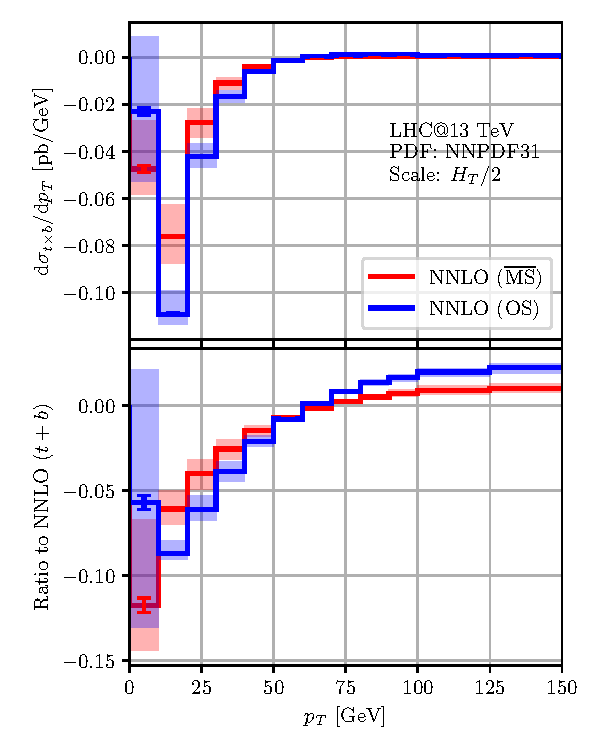
\includegraphics[width=\textwidth]{Images/pT_MS_OS_comparison_13000.pdf}
\end{minipage}
\begin{minipage}[t]{0.49\textwidth}
  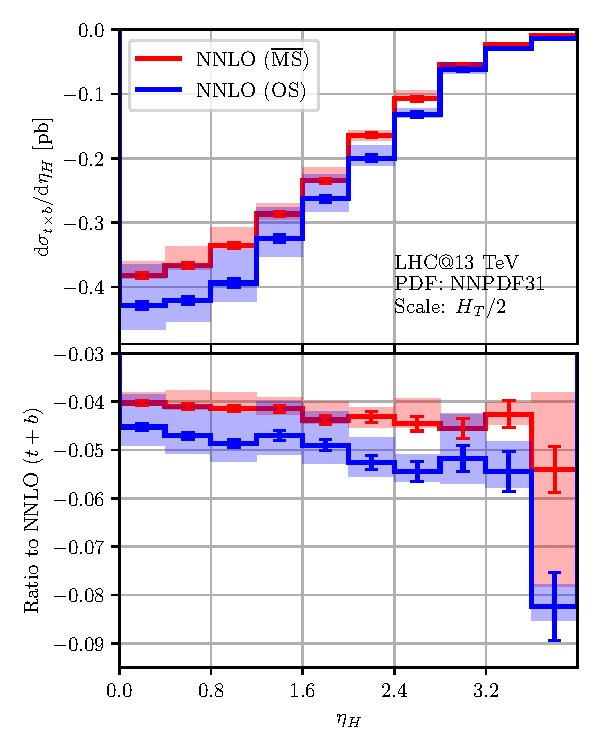
\includegraphics[width=\textwidth]{Images/yH_MS_OS_comparison_13000.pdf}
\end{minipage}
\caption{Higgs-$p_T$ (left) and Higgs-rapidity (right) distribution for the top-bottom interference contribution to the gluon-gluon-fusion cross section. Compared are the 5\acs{FS} results obtained with an \MS\ renormalized bottom-quark mass (red) against those computed with an \acs{OS} renormalized mass. The results are computed for LHC @ 13 TeV using the computational setup is described in the \hyperref[chap:notation_and_conventions]{conventions}. The transparent bands indicate the scale uncertainties, whereas the error bars show the \acs{MC} uncertainty.}
\label{fig:6:pT_yH_OS_MS_comparison}
\end{figure}
%
\begin{figure}[ht]
\begin{minipage}[t]{0.49\textwidth}
  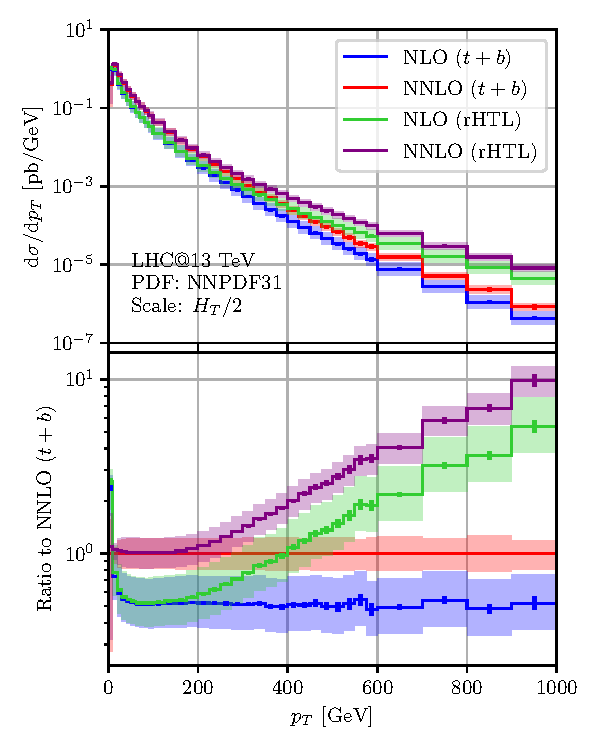
\includegraphics[width=\textwidth]{Images/pT_13000_bMS_tOS_cropped.pdf}
\end{minipage}
\begin{minipage}[t]{0.49\textwidth}
  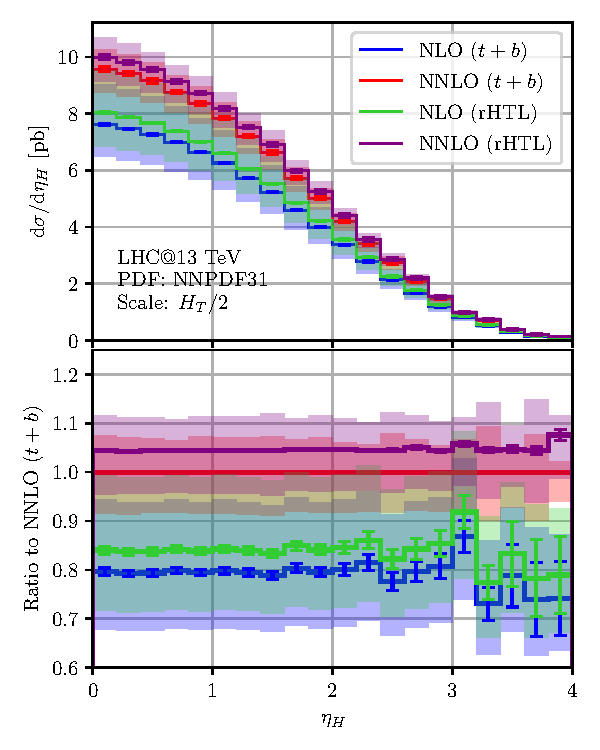
\includegraphics[width=\textwidth]{Images/yH_13000_bMS_tOS_cropped.pdf}
\end{minipage}
\caption{Higgs-$p_T$ (left) and Higgs-rapidity (right) distribution for the gluon-gluon fusion channel. Compared are the 5\acs{FS} results obtained in the \acs{rHTL} with those including finite-quark-mass effects (pure-top-quark-mass effects + top-bottom interference contribution). The bottom-quark mass is renormalized in the \MS\ scheme, while the top-quark mass is renormalized in the \acs{OS} scheme. The results are computed for LHC @ 13 TeV using the computational setup is described in the \hyperref[chap:notation_and_conventions]{conventions}. The transparent bands indicate the scale uncertainties, whereas the error bars show the \acs{MC} uncertainty.}
\label{fig:6:pT_yH_distributions}
\end{figure}
The Higgs-$p_T$ distribution is particularly interesting, as the various regions of $p_T$ are sensitive to very different physics. At large $p_T \gg m_t$, we see that the \acs{rHTL} completely breaks down and we are increasingly sensitive to finite top-quark mass effects. In Section~\ref{subsec:4:differential_cross_sections}, we explained that this is due to the non-vanishing mass dimension of coupling in of the \acs{HTL}, resulting in a less suppressed high $p_T$-tail. Our analysis concluded that the ratio of the \acs{rHTL} and \acs{SM} differential cross section must grow quadratically in $p_T$ (see Eq.~\eqref{eq:4:dSig_rHTL/dSig}). We find this rough estimate confirmed in the ratio plot of the $p_T$ distribution in Fig.~\ref{fig:6:pT_yH_distributions}. To validate this, we performed a linear fit of the logarithm of the cross-section ratio on a logarithmic $p_T$ scale. The slope of such a fit thus indicates the power of a power-law. Our fit resulted in a slope of $1.95$ within a $p_T$ range of $[500\ \mathrm{GeV}, 1000\ \mathrm{GeV}]$. If the fit is performed in a higher $p_T$ range, the slope becomes even closer to 2. The perturbative corrections are relatively constant across the spectrum for $p_T > 50\ \mathrm{GeV}$. The \acs{NNLO} correction raises the distribution by roughly a factor of two, both for the \acs{rHTL} and the \acs{SM} calculations.

At lower transverse momentum $p_T < m_t$, the top-quark running in the loop is not resolved, and the cross section is well approximated by the \acs{rHTL}. This of course excludes the effects from the missing light-quarks, which are however only relevant for $p_T < 50\ \mathrm{GeV}$. At small transverse momenta, the fixed-order cross sections are logarithmically enhanced by $\log (p_T^2/m_H^2)$, which spoil the perturbative convergence. These kinds of logarithms can be resummed to all orders of perturbation theory. For the pure-top-quark effects, the fixed order results can be compared to parton shower matched results~\cite{Niggetiedt:2024nmp}, and one observes that resummation only becomes relevant below transverse momenta of $20\ \mathrm{GeV}$. In the very low $p_T$ region where $p_T \ll m_b$, the bottom quark is not resolved and the appearing logarithms can be resummed once again. However, this region is also sensitive to non-perturbative effects~\cite{Kulesza:2003wi}. For intermediate transverse momenta  $m_b < p_T < m_H$, the top-bottom interference contribution also picks up additional logarithms of the form $\log (p_T/m_b)$ and $\log (m_H/m_b)$, potentially further degrading the perturbative convergence in this region. The origin and resummation of these are not well understood, however the resummation effects have been estimated in Ref.~\cite{Caola:2018zye}. In that reference, the authors show that the effects are only relevant for transverse momenta below 20~GeV. Coincidentally, this also marked the threshold, where the resummation of top-quark logarthims can no longer be ignored. Our fixed order results are hence reliable above this threshold.

Comparing the $p_T$-distributions of the top-bottom interference contribution computed with \acs{OS} and \MS\ renormalized bottom-quark masses (Fig.~\ref{fig:6:pT_yH_OS_MS_comparison}) reveals that the two schemes are compatible for transverse momenta above $30\ \mathrm{GeV}$. Below this threshold, we observe significant deviations and a sharp spike at around $15\ \mathrm{GeV}$ in the \acs{OS} scheme. In the \MS\ scheme the spike is also visible but less pronounced and overall there is a smoother low-$p_T$ behavior, indicating that the main improvements on the perturbative convergence over the \acs{OS} scheme come from this region of the phase-space.

The rapidity distribution is not subject to logarithmic enhancements and remains reliable across the entire range. The distribution overall is less feature rich. With an \MS\ renormalized bottom-quark mass, the top-bottom interference contribution approximately results in a shift of $-4\%$ across the entire rapidity spectrum. In the \acs{OS} scheme the shift is slightly larger---around $-4.5\%$ with a slight negative tilt towards larger rapidities. Relative scale uncertainties remain roughly constant and are significantly larger in the \acs{OS}-scheme, as expected from our findings on the total cross section (see Tab.~\ref{tab:6:top-bottom}). In the right panel of Fig.~\ref{fig:6:pT_yH_distributions}, we can see that the \acs{NNLO} corrections on the total cross section result in a shift of $+20\%$ across the entire rapidity spectrum, both for the \acs{rHTL} and the \acs{SM} cross section. This once again perfectly aligns with the observed corrections in the total cross section in Tab.~\ref{tab:6:t-HEFT}. Similarly, the \acs{rHTL} differential cross section overshoots the full cross section by around $4-5\%$ across the entire spectrum, aligning perfectly with the observed shift of the top-bottom interference contribution in the right panel Fig.~\ref{fig:6:pT_yH_OS_MS_comparison}.

\section{Validation \& Comparison With Other Works}
In the 4\acs{FS}, the bottom-quark mass acts as an \acs{IR}-regulator, resulting in huge logarithmic enhancements of the individual amplitudes. To check that these enhancements cancel in inclusive observables, we performed the calculation of the \acs{rHTL} cross section for a number of small bottom-quark masses. This means that the cross section contains only contributions arising from the effective coupling of the Higgs to gluons, and the bottom-quark mass is only relevant in bottom-quark loops which are not coupling to the Higgs. These loops, however, are precisely the ones that give rise to the logarithmic enhancements. The results are displayed in Tab.~\ref{tab:6:rHTL_4fs}.
\begin{table*}[h]
\centering
\begin{tabular}{cccccc}
\hline
Order & \multicolumn{5}{c}{$\sigma_\text{rHTL}$ [pb]} \\
\hline
\hline
\multicolumn{6}{c}{$\sqrt{s}=13$~TeV} \\
\hline
& 5FS & 4FS  & 4FS & 4FS & 4FS  \\
& & $m_b=0.01$~GeV &  $m_b=0.1$~GeV & $m_b=4.78$~GeV & $\overline{m}_b(\overline{m}_b) = 4.18$ GeV \\
\hline
$\mathcal{O}(\alpha_s^2)$ & $+16.30$ & +16.27 & +16.27 & +16.27 & $16.27$\\
LO & $16.30^{+4.36}_{-3.10}$ & $16.27^{+4.63}_{-3.22}$ & $16.27^{+4.63}_{-3.22}$ & $16.27^{+4.63}_{-3.22}$ & $16.27^{+4.63}_{-3.22}$ \\
\hline
$\mathcal{O}(\alpha_s^3)$ & +21.14 & +20.08(3) & +20.08(3) & +20.08(3) & +20.08(3) \\
NLO & $37.44^{+8.42}_{-6.29}$ & $36.35(3)^{+8.57}_{-6.32}$ & $36.35(3)^{+8.57}_{-6.32}$ & $36.35(3)^{+8.57}_{-6.32}$ & $36.35(3)^{+8.57}_{-6.32}$ \\
\hline
$\mathcal{O}(\alpha_s^4)$ & +9.72 & +10.8(4) & +11.1(4) & +9.5(2) & $+9.6(2)$ \\
NNLO & $47.16^{+4.21}_{-4.77}$ & $47.2(4)^{+5.4}_{-5.4}$ & $47.5(4)^{+5.4}_{-5.5}$ & $45.9(2)^{+4.3}_{-4.9}$ & $46.0(2)^{+4.4}_{-5.0}$\\
\hline
\end{tabular}
\caption{rHTL cross section in the 5-flavour scheme and for different bottom-quark masses in the 4-flavour scheme. In the last column the cross section and the scale variation are computed with the $\overline{\text{MS}}$-mass. The results are computed for LHC @ 13 TeV using the computational setup is described in the \hyperref[chap:notation_and_conventions]{conventions}. The scale uncertainties are determined with seven-point variation. Numbers in parentheses indicate the \acs{MC} uncertainties on the last provided digit. Results computed in the 5\acs{FS} were computed using \texttt{SusHi}.}
\label{tab:6:rHTL_4fs}
\end{table*}
The results clearly show that there are no logarithmic enhancements on the cross section level, as there is no pronounced rise of the cross section for decreasing bottom-quark masses. We further observe that the 4\acs{FS} results approach the 5\acs{FS} results in the limit $m_b \rightarrow 0$. For realistic values of the bottom-quark mass (last two columns in Tab.~\ref{tab:6:rHTL_4fs}), we see a significant change from the 5 to the 4\acs{FS} of around $-2\%$, which is, however, still well within the associated scale uncertainties. Finally, results for \acs{OS} and \MS\ renormalized bottom-quark masses show no significant deviations.

To further validate our findings, we compared our $p_T$ spectra against existing Higgs+jet analysis. The top-bottom interference contribution with \acs{OS}-renormalized top- and bottom-quark masses was compared to the results presented in Ref.~\cite{Caola:2018zye}. In that reference, the authors approximate the real-virtual corrections using the \acs{HTL} for the top-quark, and they work under the assumption of a nearly massless bottom-quark. Fig.~\ref{fig:6:caola_comparison} shows the comparison of the two results. We see that the approximations perform well for transverse momenta below $40\ \mathrm{GeV}$, but result in an error of about $20\%$ above this threshold. Since the approximation of a nearly massless bottom quark is expected to perform well in the limit $m_b \ll m_H, p_T$, the discrepancy is likely due to the \acs{HTL} approximation. Since the $p_T$ range $[0, 40\ \mathrm{GeV}]$ is responsible for the majority of the top-bottom interference contribution---about 99\%---, the approximation is still highly accurate for the total cross section. Additionally, we observe that the scale uncertainties of the first two bins are significantly larger in Ref.~\cite{Caola:2018zye}. We were able to identify that this difference arises only from a single scale variation ($\mu_R/\mu = 1, \mu_F/\mu = 2)$, but we have not found any error on our end that would account for this difference.
\begin{figure}[h]
\centering
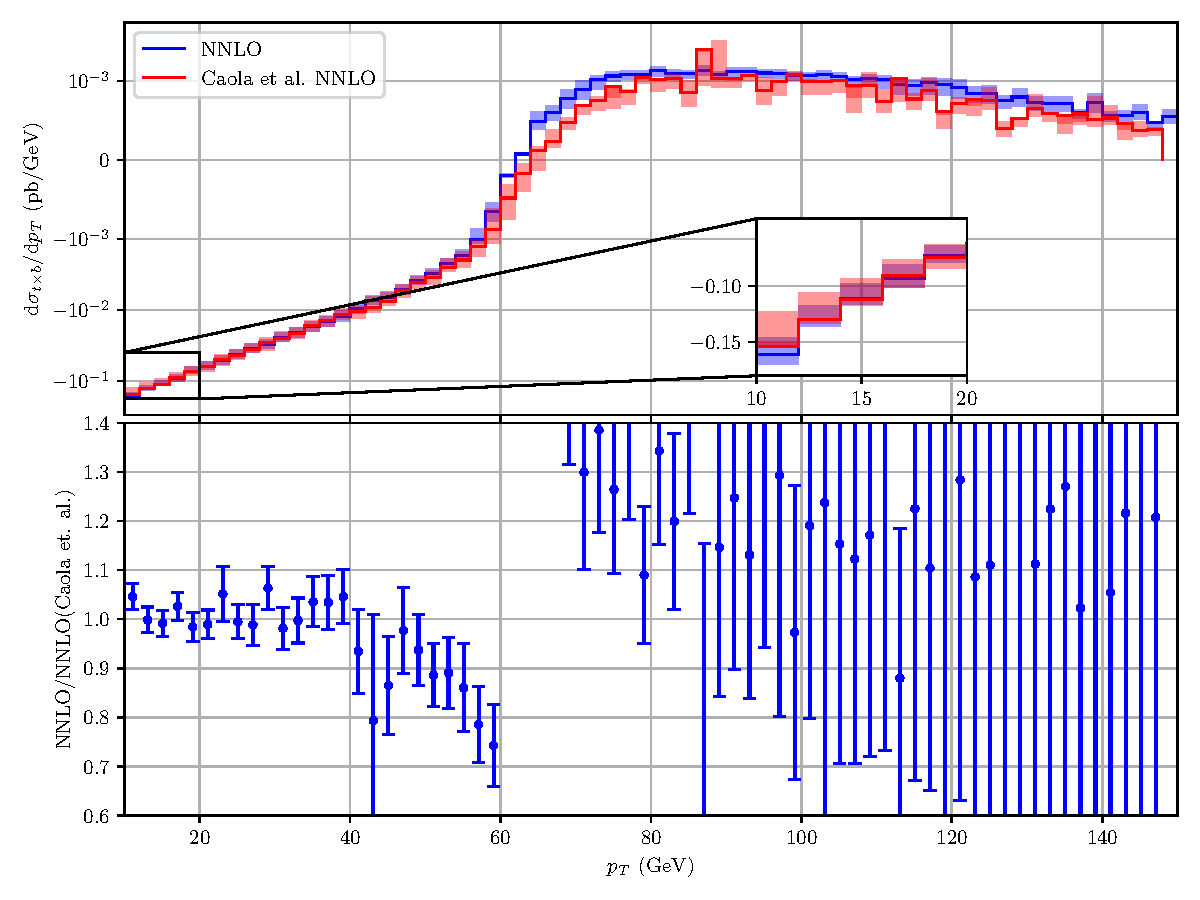
\includegraphics[width=\figurewidth]{Images/Caola_comparison}
\caption{Top-bottom interference contribution to the Higgs production cross section. Displayed are our results and the results presented in Ref.~\cite{Caola:2018zye}, with data provided by the authors. The authors of that reference used an \acs{OS} top- and bottom-quark mass of $m_t = 173.2\ \mathrm{GeV}$, and $m_b = 4.75\ \mathrm{GeV}$, whereas we used $m_t = 173.05\ \mathrm{GeV}$ and $m_b = 4.78\ \mathrm{GeV}$ and the same Higgs mass of $m_H = 125\ \mathrm{GeV}$. For the sake of this comparison, we used the same \texttt{PDF4LHC15\_nlo\_30} \acs{PDF} set and a central scale of $\mu = \frac{1}{2}\sqrt{m_H^2 + p_T^2}$. The transparent bands indicate scale uncertainties, whereas the error bars in the lower panel indicate the \acs{MC} uncertainties dominated by the uncertainties of Ref.~\cite{Caola:2018zye}.}
\label{fig:6:caola_comparison}
\end{figure}

Furthermore, we compared our findings of the pure-top and the top-bottom-interference contribution with both quark-masses defined in the \MS\ scheme with the results presented in Ref.~\cite{Bonciani:2022jmb}.
\begin{figure}[h]
\centering
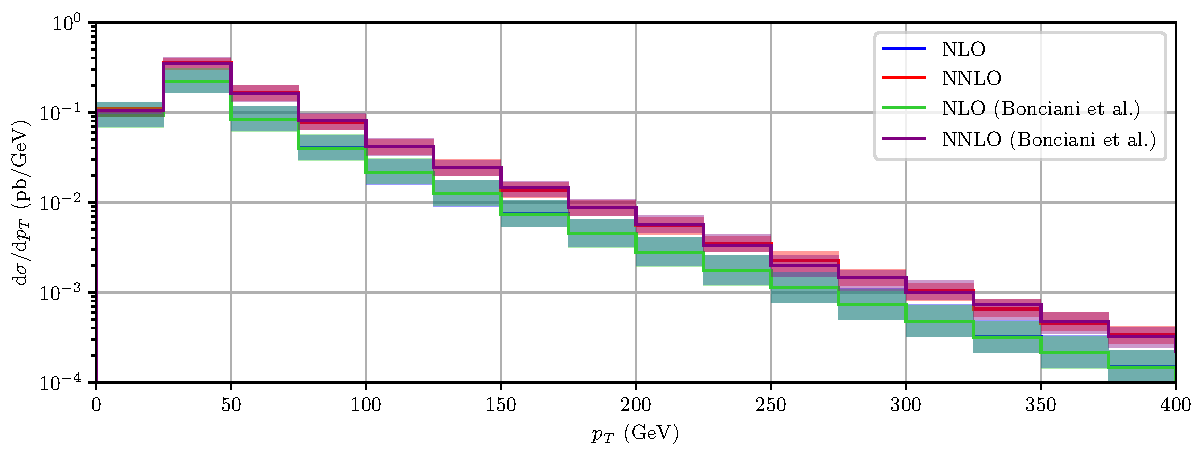
\includegraphics[width=\textwidth]{Images/pTBonciani.pdf}
\caption{Comparison of the differential cross section of the gluon-gluon fusion channel between our findings and the results presented in Ref.~\cite{Bonciani:2022jmb}. The cross section constitutes the pure-top-quark, the top-bottom interference, and the pure-bottom-quark contribution, however, we neglect the pure-bottom-quark contribution for all \acs{NNLO} corrections. For the sake of this comparison we use the same computational setup as the authors of Ref.~\cite{Bonciani:2022jmb}, namely top- and bottom-quark masses defined in the \MS\ scheme with the masses $\msMass{t} = 163.4\ \mathrm{GeV}$ and $\msMass{b} = 4.18\ \mathrm{GeV}$. The running of the quark-masses is computed at two-loop accuracy. The Higgs mass is set to $m_H = 125.25\ \mathrm{GeV}$. We apply the anti-$k_T$ algorithm with a jet radius of $R = 0.4$ and use the central scale $\mu = \frac{1}{2}\left( \sqrt{m_H^2 + p_T^2} + \sum_i p_{i, T} \right)$, where the sum runs over all jet momenta. We use a $p_T$-cut on the jets, requiring that at least one of the jets satisfies $p_{i,T} > 20 \ \mathrm{GeV}$. We use the \texttt{NNPDF40\_nlo\_as\_01180} \acs{PDF} set.}
\label{fig:6:bonciani_comparison}
\end{figure}
The results show excellent agreement for transverse momenta $p_T \le 400 \ \mathrm{GeV}$. Above this scale we find significant deviations. We were able to identify that the problem arises from the real-virtual amplitudes. Indeed, our numerical grids were only computed for top-quark masses up to a scale of $\mu_R = 125\ \mathrm{GeV}$. If the scale exceeds this value, we are extrapolating from our grid. This then results in large errors for $p_T > 400 \ \mathrm{GeV}$. We stress that all our previous findings did not rely on this extrapolation, since we used fixed scales whenever we renormalized the top-quark mass in the \MS\ scheme.

\section{Recommendations for Phenomenological Applications} \label{sec:6:recommendations}
We conclude this chapter by giving our recommendations for the total gluon-gluon fusion Higgs-production cross section for future phenomenological applications. We combine our findings with the full \NNNLO\ \acs{rHTL} results, the partial $\mathrm{N}^4\mathrm{LO}$ results in the soft-virtual approximation, the available electroweak corrections, and the finite top-quark mass effects. The associated uncertainties of each contribution are carefully examined.

Following our discussion of Section~\ref{subsec:4:scale_uncertainties}, we suggest using $\mu = m_H/2$ as the central scale. Moreover, we recommend using the \texttt{MSHT20xNNPDF40\_aN3LO} \acs{PDF} set until full \NNNLO\ sets become available.

The top-bottom interference contribution proved to be quite independent of the chosen \acs{FS}. We therefore suggest using the 5\acs{FS} going forward, because large logarithms are automatically resummed in this \acs{FS} by the running of the \acs{PDF}s. The renormalization scheme of the top-quark mass also did not affect the cross section significantly. Both the \MS\ and the \acs{OS} scheme are therefore valid choices. In the following we provide results for the latter. The bottom-quark mass on the other hand, was very sensitive to the renormalization scheme, and the \MS\ scheme showed significantly better perturbative convergence, which is why we strongly recommend using this scheme from now on.

Our best prediction for the gluon-gluon fusion cross section is
\begin{equation}
\begin{alignedat}{4}
\sigma_{pp \rightarrow HX} (13\ \mathrm{TeV}) = +\ & 15.33 \ &&\mathrm{pb    } && (+33.17\%) \quad  &&(\text{LO rHTL}) \\
+\ & 19.99\ &&\mathrm{pb} \quad && (+43.26\%)  &&(\text{NLO cor.\ rHTL}) \\
+\ & 9.20\ &&\mathrm{pb} \quad && (+19.91\%) &&(\text{NNLO cor.\ rHTL}) \\
+\ & 1.56\ &&\mathrm{pb} \quad && (+3.38\%) &&(\text{N}^3\text{LO cor.\ rHTL}) \\
+\ & 0.14\ &&\mathrm{pb} \quad && (+0.30\%) &&(\text{N}^4 \text{LO cor.\ rHTL in s.-v.\ approx.}) \\
+\ & 2.02\ &&\mathrm{pb} \quad && (+4.37\%) &&(\text{NLO EW-QCD}) \\
-\ & 0.16\ &&\mathrm{pb} \quad && (-0.35\%) &&(\text{NNLO finite top-quark mass}) \\
-\ & 0.23\ &&\mathrm{pb} \quad && (-0.50\%) &&(\text{NLO top-charm interference}) \\
+\ & 0.10 \ &&\mathrm{pb}\quad && (+0.22\%) &&(\text{NLO pure bottom-quark effects}) \\
-\ & 1.74\ &&\mathrm{pb} \quad && (-3.77\%) &&(\text{NNLO cor.\ top-bottom interference}) \\[-10pt]
& &&  \hspace{0.5cm} \mathclap{\rule{4.5cm}{0.4pt}}\\[-4pt]
& 46.21 \ &&\mathrm{pb} && (100\%).
\end{alignedat}
\end{equation}
Here, ``cor.'' refers to the correction of the respective perturbative order. The \acs{rHTL} results were computed using \texttt{iHixs 2}. The N${}^4$LO results were extracted from the $K$-factor with respect to \NNNLO\ at 13~TeV, provided in Ref.~\cite{Das:2020adl}. In that reference the authors use a slightly altered computational setup, including a different \acs{PDF} (\texttt{MMHT2014}). Since the N${}^4$LO corrections are tiny, the final result should not be affected by this significantly. Similarly, the electroweak corrections were extracted from Ref.~\cite{Becchetti:2020wof}, where the authors used the \texttt{PDF4LHC15\_nlo\_30} PDF set and slightly different masses for the Higgs, and the top- and bottom-quark\footnote{The authors also used a bottom-quark mass defined in the \acs{OS} scheme.}. Once again, the electroweak corrections themselves are small, making the impact of a slightly altered computational setup non-essential. Finally, the effects from finite top- and bottom-quark masses were computed using the \texttt{NNPDF31\_nnlo\_as\_0118} PDF set.

We estimate the \acs{MHOU}, based on the $\mu_R$ variation\footnote{Recently, the \acs{MHOU} were also estimated using theory nuisance parameters~\cite{Lim:2024nsk} at \acs{NNLO}. The authors found the uncertainties to be compatible.} of the N${}^4$LO cross section in the soft-virtual approximation in the range $[m_H/4, m_H]$ presented in Ref.~\cite{Das:2020adl}. The factorization scale dependence was shown to be very small (see Fig.~\ref{fig:4:scale_scan}), making it an accurate estimate of \acs{MHOU}. We can estimate the error of the soft-virtual approximation itself based on lower orders. We conservatively assign the uncertainty by taking the perturbative order at which the soft-virtual approximation yielded the worst estimate of the perturbative correction and then apply the resulting accuracy to the N${}^4$LO results
\begin{equation}
\delta(\Delta  \sigma^{\text{N}^4\text{LO}}_{\text{s.-v.}}) = \left(\text{max} \lbrace \sigma^{\text{NLO}}_\text{rHTL}/\sigma^{\text{NLO}}_{\text{s.-v.}},\sigma^{\text{NNLO}}_\text{rHTL}/\sigma^{\text{NNLO}}_{\text{s.-v.}},  \sigma^{\text{N}^{n-1}\text{LO}}_\text{rHTL}/\sigma^{\text{N}^{n-1}\text{LO}}_{\text{s.-v.}} \rbrace - 1 \right) \Delta  \sigma^{\text{N}^n\text{LO}}_{\text{s.-v.}}.
\end{equation}
Here, $\Delta \sigma^{\text{N}^n\text{LO}}_{\text{s.-v.}}$ refers to the correction of the cross section at $\text{N}^n\text{LO}$.
Uncertainties on the electroweak corrections are also dominated by \acs{MHOU}, and we adopt the uncertainties assigned in Ref.~\cite{Becchetti:2020wof}. Errors associated with missing higher orders in the \acs{PDF} fits, including the missing ingredients for the DGLAP evolution equation, are estimated by comparing cross section results computed using the \texttt{NNPDF40\_an3lo\_as\_01180\_mhou} and the \texttt{NNPDF40\_an3lo\_as\_01180} \acs{PDF} set, \ie\ the uncertainty is calculated via
\begin{equation}
\delta (\text{PDF MHOU}) = \sqrt{\left(\sigma_{gg \rightarrow HX}^\mathtt{NNPDF40\_an3lo\_as\_01180\_mhou} \right)^2 - \left(\sigma_{gg \rightarrow HX}^\mathtt{NNPDF40\_an3lo\_as\_01180} \right)^2}.
\end{equation}
This assumes that the \acs{PDF}-theory and the \acs{PDF} uncertainties are uncorrelated. Uncertainties for finite quark-mass effects are determined through seven-point scale variation. The full theory uncertainty can be broken down as follows:
\begin{equation}
\begin{alignedat}{5}
\delta(\text{theory}) =\ \  & {}^{+0.10}_{-1.73}\ &&\text{pb    }  && ({}_{-3.7\%}^{+0.2\%}) \quad  &&(\text{scale}) \\
\pm & 0.24\ &&\mathrm{pb}  && (\pm 0.5\%) &&(\text{s.-v.\ approx.}) \\
\pm & 0.14\ &&\mathrm{pb}  && (\pm 0.3\%) &&(\text{electroweak}) \\
\pm & 0.16\ &&\mathrm{pb} && (\pm 0.3\%) &&(\text{PDF MHOU}) \\
& {}^{+0.13}_{-0.03}\ &&\mathrm{pb}  && ({}_{-0.1\%}^{+0.3\%}) &&(\text{finite top-quark mass}) \\
& {}^{+0.13}_{-0.03}\ &&\mathrm{pb}  && ({}_{-0.1\%}^{+0.3\%}) &&(\text{top-bottom interference}) \\[-10pt]
& && \hspace{0.3cm} \mathclap{\rule{3.2cm}{0.4pt}}\\[-4pt]
& {}^{+0.35}_{-1.76}  \ &&\mathrm{pb} && ({}_{-3.8\%}^{+0.8\%}).
\end{alignedat}
\end{equation}
For the final theory uncertainty, we added all individual errors in quadrature. In Section~\ref{subsec:4:effect_of_light_quarks} we observed that the top-bottom interference contribution is actually anti-correlated with the pure-top-quark contribution. We do not take this anti-correlation into account here, because the correlations among the other sources of uncertainty are currently unavailable. The error budget is illustrated in Fig.~\ref{fig:6:error_budget}.
\begin{figure}[h]
\centering
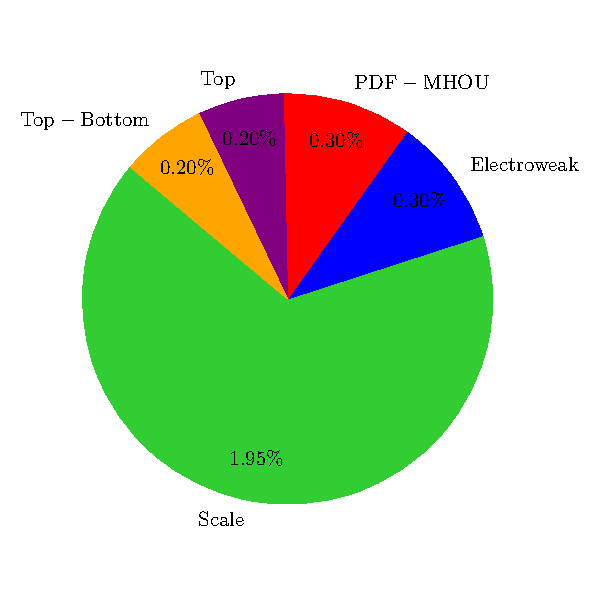
\includegraphics[scale=0.8]{Images/error_budget_after.pdf}
\caption{Total error budget of the fully inclusive gluon-gluon fusion Higgs production cross section at 13~TeV. Uncertainties are assigned as described in the text.}
\label{fig:6:error_budget}
\end{figure}

The uncertainty estimates are slightly different from the upcoming Higgs Working Group recommendation~\cite{Cappati:2024}, mainly due to the fact that electroweak corrections are not incorporated with full \acs{NLO} precision. Furthermore, the Higgs Working Group assumes maximal correlation among the various uncertainties. The uncertainty estimates presented here are therefore smaller by approximately $1\%$ of the total cross section.

Finally, the uncertainties on the \acs{PDF} sets are combined with the $\alphas$ uncertainties, assuming that the errors are uncorrelated. This not entirely realistic assumption, is adopted out of necessity, since the \texttt{MSHT20xNNPDF40\_aN3LO} \acs{PDF} set does not support correlations yet. The $\alphas$-uncertainty is estimated by reevaluation of the \NNNLO\ \acs{rHTL} cross section at $\alphas (m_Z) = 0.117$ and $\alphas (m_Z) = 0.119$, corresponding to the standard deviation of $\alphas$~\cite{ParticleDataGroup:2022pth}, the resulting range is taken as the standard deviation. The combined uncertainty reads
\begin{equation}
\begin{split}
\delta (\text{PDF} + \alphas) &= \sqrt{\left[\delta (\text{PDF}) \right]^2 + \left[\delta (\alphas)\right]^2} = \sqrt{\left[0.88\ \text{pb}\ (1.9\%) \right]^2 + \left[{}^{+1.23}_{-1.21} \ \text{pb}\ ({}^{+2.6\%}_{-2.6\%}) \right]^2} \\
&= {}^{+1.52}_{-1.50}\ \text{pb} \ ({}^{+3.3\%}_{-3.2\%}).
\end{split}
\end{equation}

Our final best prediction for the gluon-gluon fusion cross at 13~TeV is
\begin{equation}
\boxed{\sigma_{pp \rightarrow HX} (13 \ \mathrm{TeV}) =  46.21^{+0.35}_{-1.76}\ (\text{theory})\ {}^{+1.52}_{-1.50}\ (\text{PDF} + \alphas) \ \text{pb}. }
\end{equation}
This is in excellent agreement with the current best measurement of the cross section~\eqref{eq:2:xSec_pp2H_experiment}.



